\section{Data partitioning}

The spatial indices structure can be derived either from one-dimensional structures (such as a grid file) or from ad-hoc structures (like an R-tree), resulting in a myriad of potential data structures.
\begin{figure}[H]
    \centering
    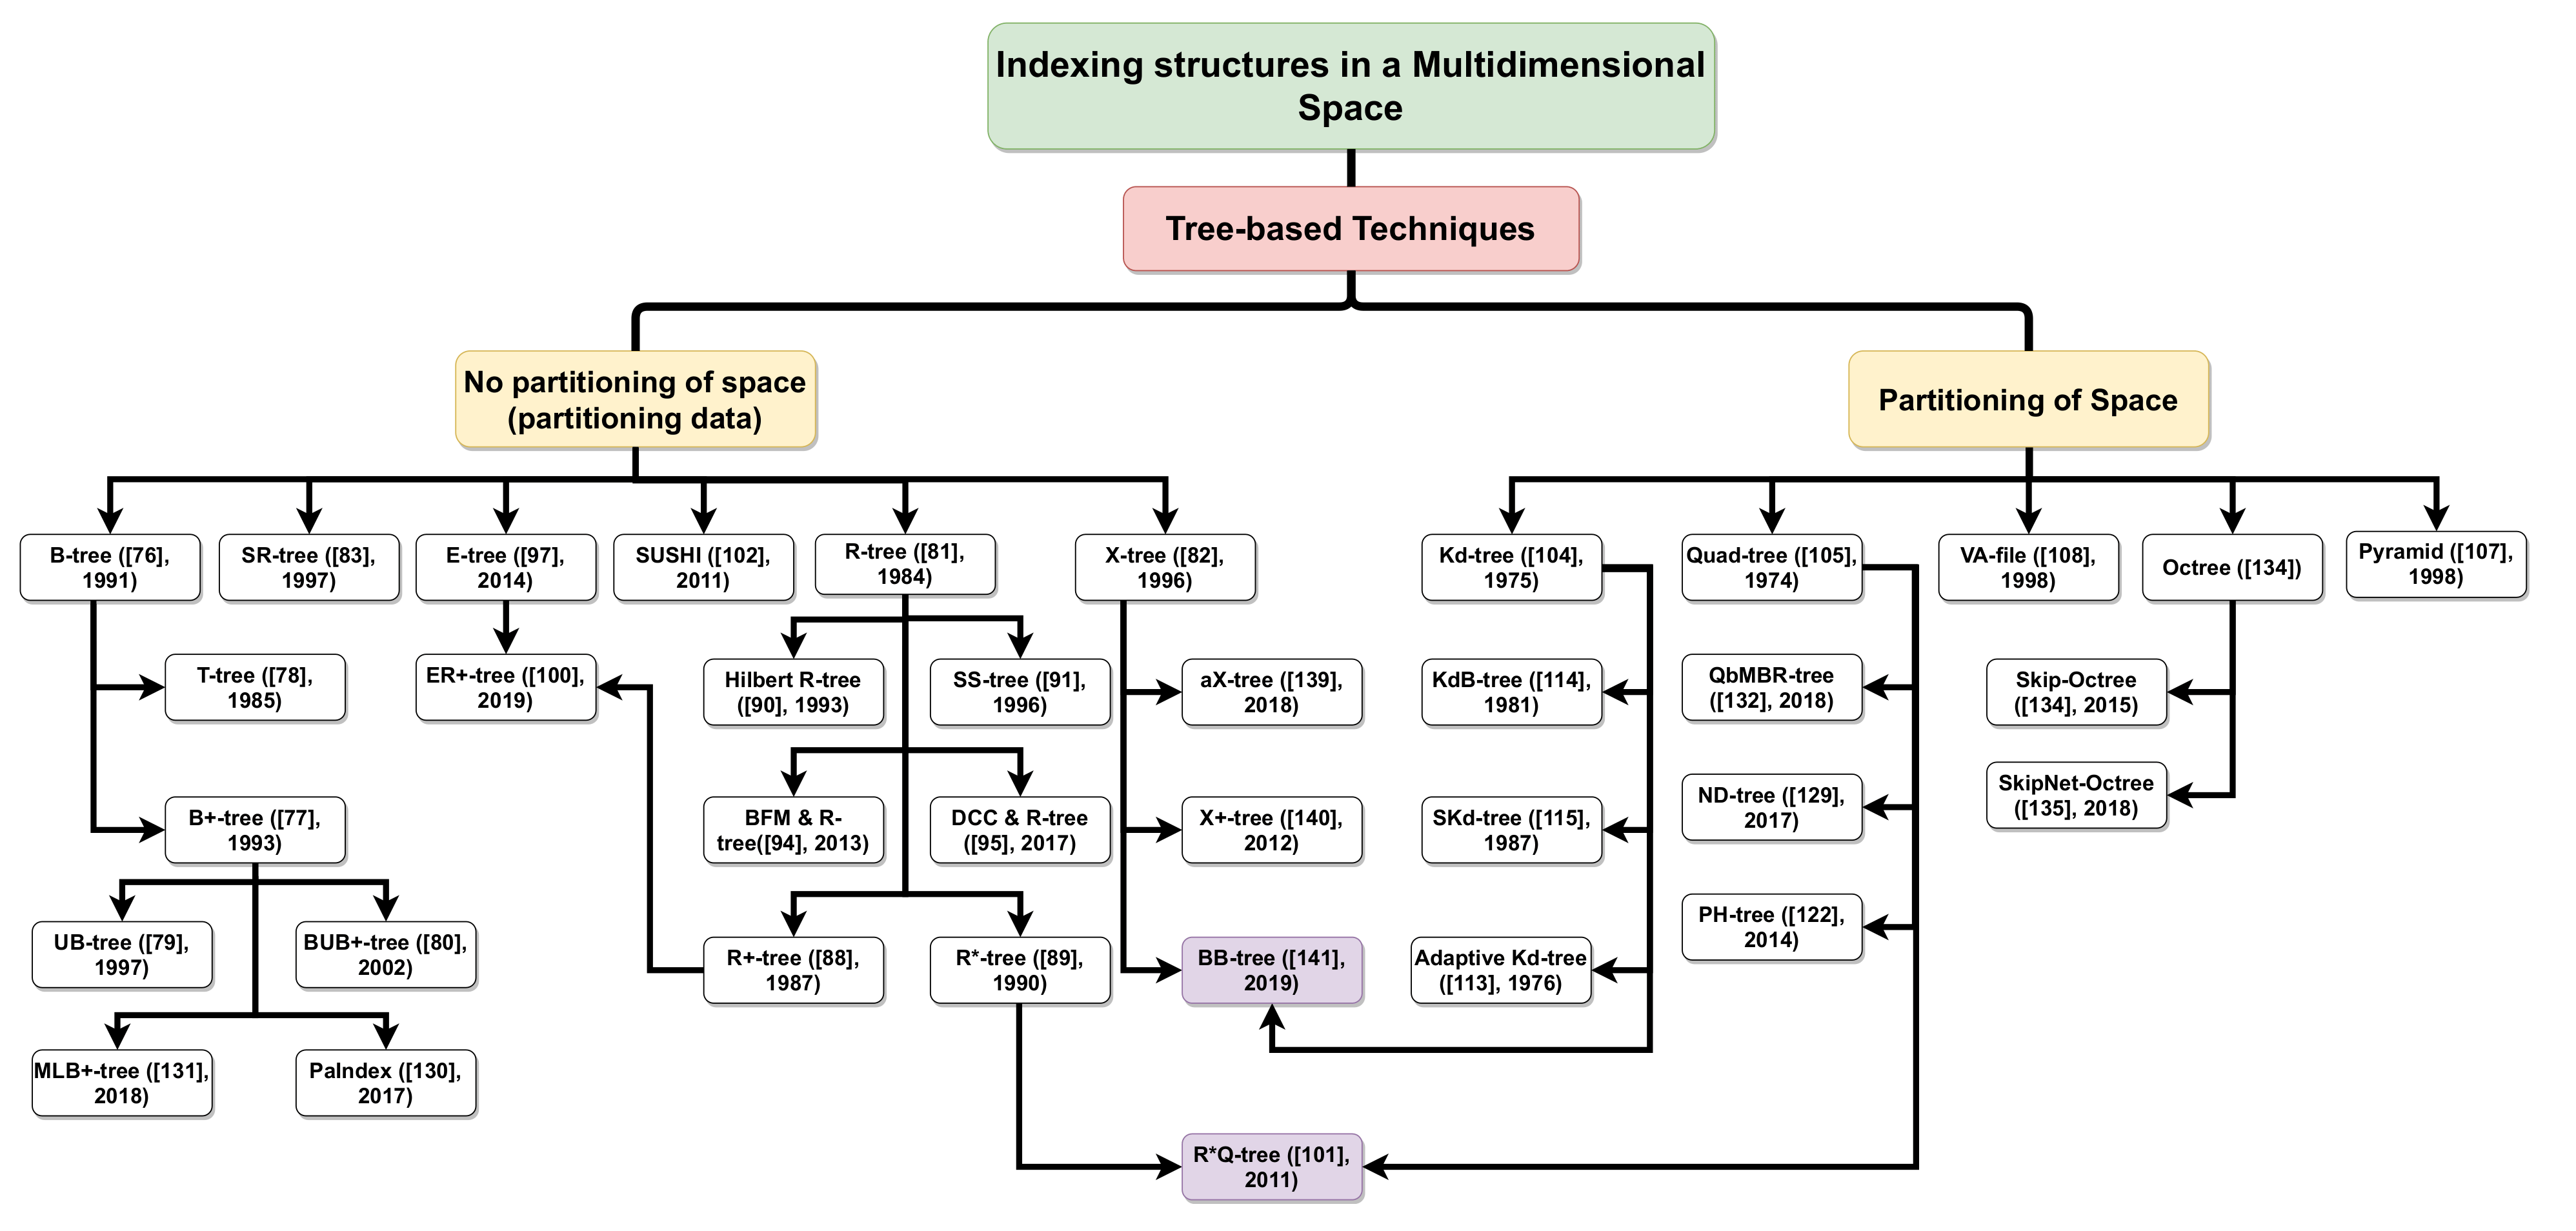
\includegraphics[width=1\linewidth]{images/mult.png}
    \caption{Taxonomy of tree-based indexing techniques}
\end{figure}

\paragraph*{Classification}
Spatial indices can be classified based on:
\begin{itemize}
    \item \textit{Type of objects}: points, lines, and regions. 
    \item \textit{Type of subdivision}: 
        \begin{itemize}
            \item Space partitioning: splits are executed according to global considerations, which is beneficial for uniform distributions and easier to implement.
            \item Data partitioning: splits are performed based on local considerations, akin to B+-trees. 
                This method is suitable for arbitrary distributions but is more complex to implement.
        \end{itemize}
    \item \textit{Type of organization}: either tree-based or hash-based. 
\end{itemize}
The prevalent approach involves organizing space into regions, referred to as cells, where each cell corresponds to a data page (although this correspondence is not always one-to-one).

\subsection{Grid files}
The Grid file arranges the spatial domain into a grid, with each dimension divided into intervals of arbitrary sizes. 
This entails the use of $d$ scales (monodimensional arrays) that hold values serving as separators for each dimension. 
Each grid cell is linked to a data page on disk, allowing for the possibility of two or more cells sharing the same data page.
\begin{figure}[H]
    \centering
    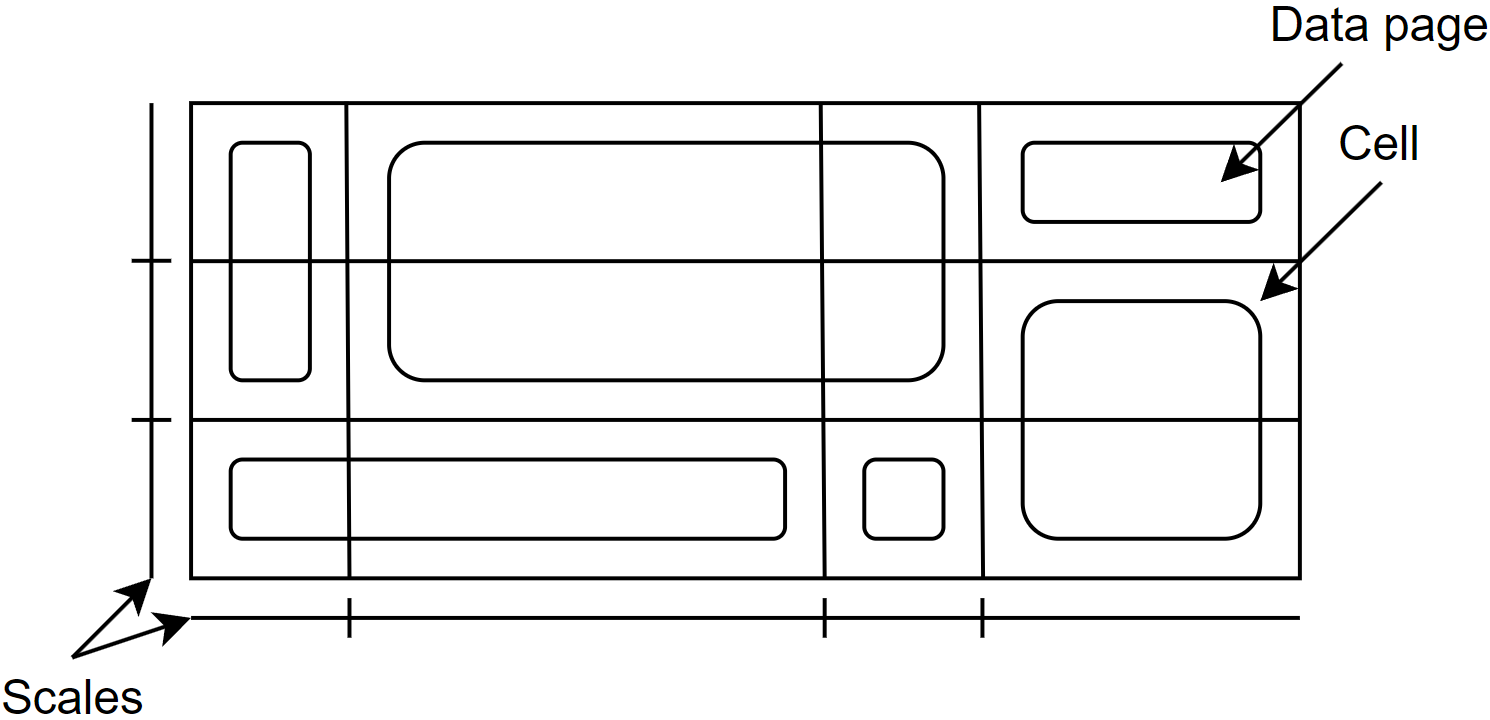
\includegraphics[width=0.5\linewidth]{images/grid.png}
\end{figure}
When a data page reaches its capacity and overflows, it undergoes a split.
After a split, the directory structure changes by applying one of the following actions: 
\begin{itemize}
    \item If the block was referenced by two or more cells, we simply update the pointers.
    \item Otherwise, if the block was referenced by a single cell, we add a separator to the directory.
\end{itemize} 
\begin{example}
    Examine the given directory:
    \begin{figure}[H]
        \centering
        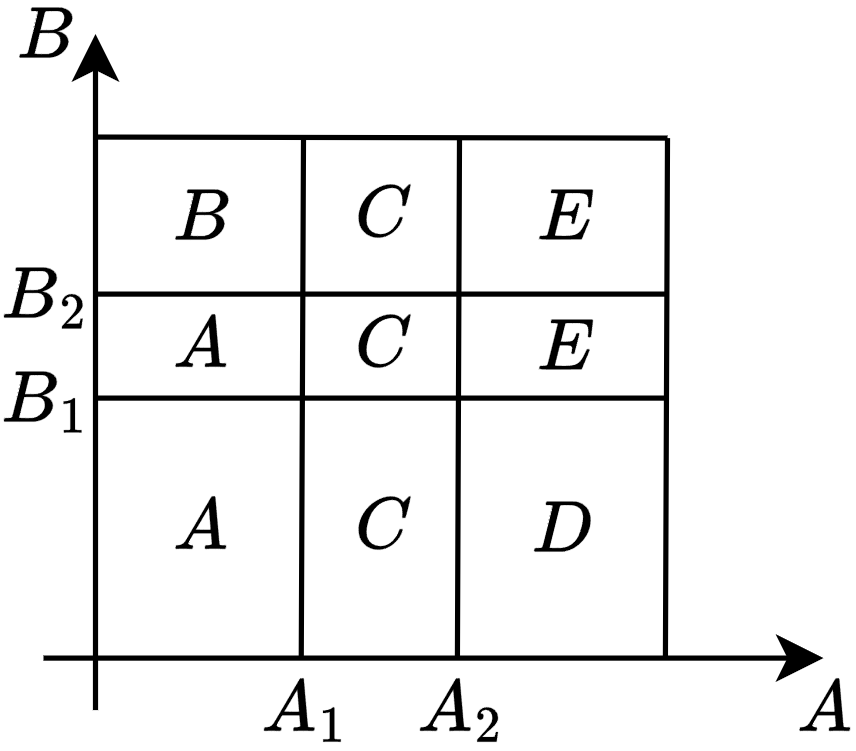
\includegraphics[width=0.25\linewidth]{images/grid1.png}
    \end{figure}
    Associated with the depicted data pages below:
    \begin{figure}[H]
        \centering
        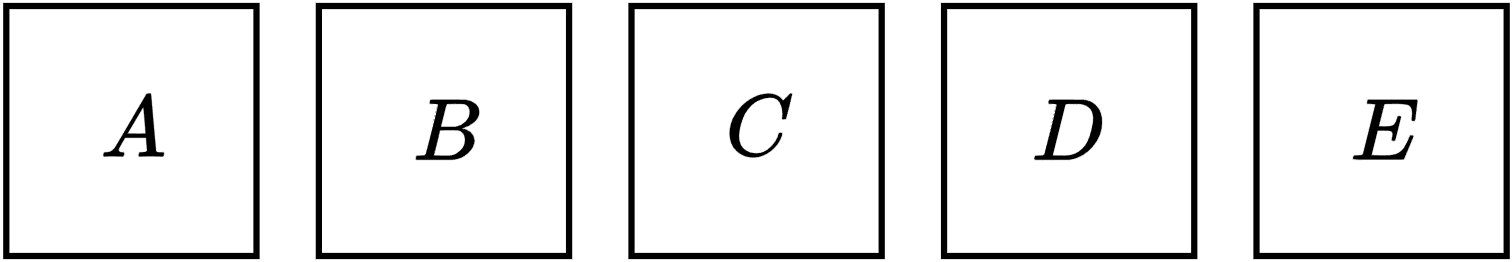
\includegraphics[width=0.4\linewidth]{images/grid2.png}
    \end{figure}
    Now, consider the scenario where $C$ overflows and undergoes a split into $C$ and $F$. 
    In this case, it is sufficient to update the pointer of the cell. 
    The resulting directory and data pages are as follows:
    \begin{figure}[H]
        \centering
        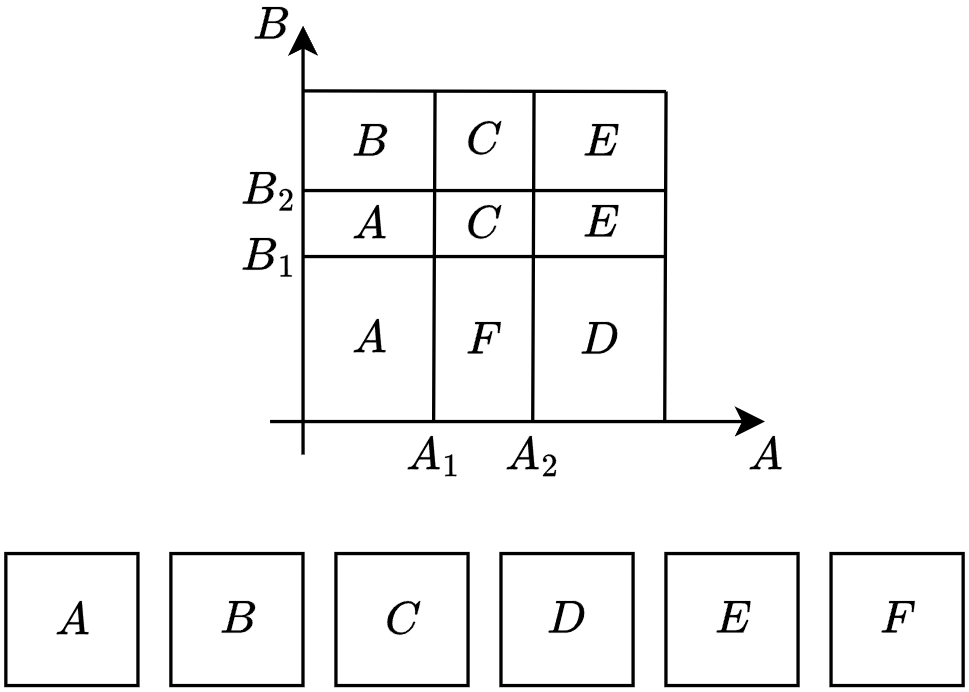
\includegraphics[width=0.5\linewidth]{images/grid3.png}
    \end{figure}
    Next, consider the case where $D$ overflows and is split into $D$ and $G$. 
    In this scenario, we need to augment the directory using an additional separator for coordinate $A$. 
    The resulting directory and data pages become:
    \begin{figure}[H]
        \centering
        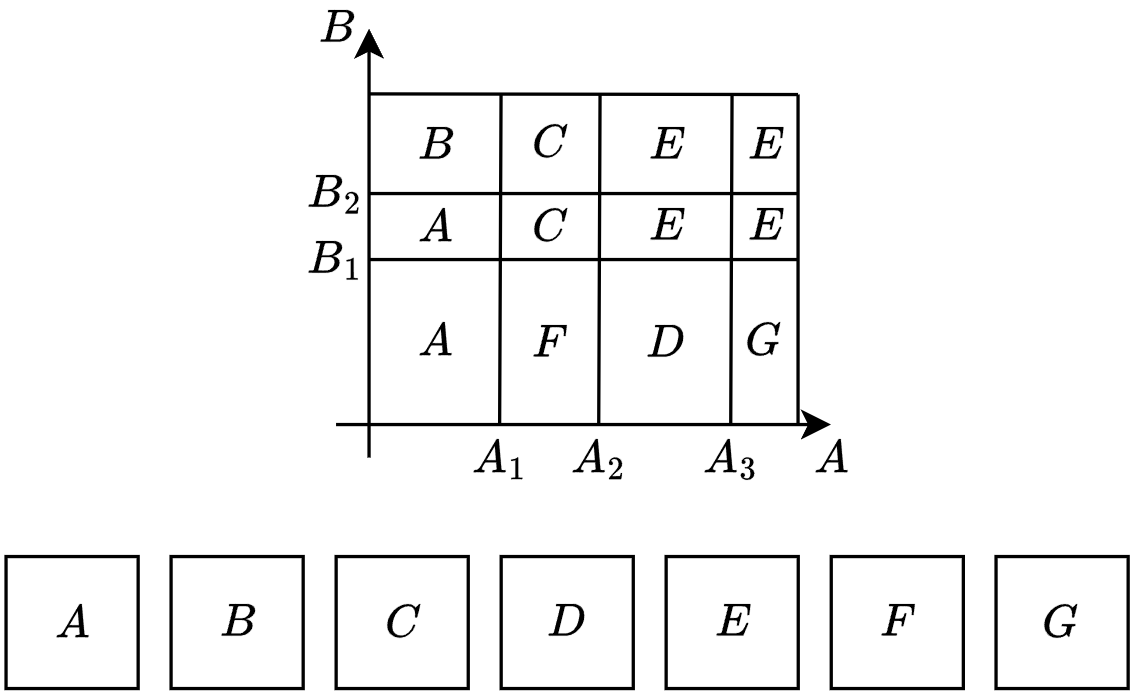
\includegraphics[width=0.6\linewidth]{images/grid4.png}
    \end{figure}
\end{example}

\paragraph*{Summary}
For non-uniform distributions, the storage of $n$ points may demand a number of cells that increases proportionally to $O(n^d)$.
In general, this approach exhibits poor performance with correlated data.
Conversely, the structured nature of space partitioning significantly simplifies the resolution of window queries.

The primary challenge with this technique lies in the management of the directory. 
Typically, scales are stored in main memory.
In quasi-static scenarios, the directory can be stored on disk as a multidimensional array.
However, in dynamic cases, it becomes essential to paginate the directory, resulting in multi-level grid files.

\subsection{R-tree}
An R-tree is a well-balanced and paginated tree structure built upon the hierarchical nesting of overlapping regions.
In this structure, every node represents a rectangular region, specifically the Minimum Bounding Box (MBB) encapsulating its children's regions.
The storage utilization for each node ranges from 100\% down to a minimum value ($\leq$ 50\%), a parameter set during design.
The management mechanisms in an R-tree bear similarities to those found in a B+ tree. 
However, a key distinction lies in the fact that the insertion of an object and splits can be handled according to different policies.

\paragraph*{Minimum Bounding Box}
The Minimum Bounding Box is the smallest rectangle containing all children regions, with sides parallel to the coordinate axes.
It is determined by the product of $d$ intervals and can be uniquely defined by the (2d) coordinates of any two opposite vertices, typically the lower-left and upper-right vertices.
The computation of the MBB for $m$ points in $d$ dimensions can be performed in $O(md)$ time.
\begin{figure}[H]
    \centering
    \includegraphics[width=0.5\linewidth]{images/MBB.png}
    \caption{Graphical representation of a 2d and a 3d MBB}
\end{figure}
The differences between a B+ tree and an R-tree are outlined below: 
\begin{table}[H]
    \centering
    \begin{tabular}{ll}
    \hline
    \multicolumn{1}{c}{\textbf{B+ tree}}                                                & \multicolumn{1}{c}{\textbf{R-tree}}                                                               \\ \hline
    Balanced and paginated tree                                                         & Balanced and paginated tree                                                                       \\
    Data are stored in leaves                                                           & Data are stored in leaves                                                                         \\
    Leaves are kept sorted and linked                                                   & No data order exist                                                                               \\
    Data are organized into 1D intervals                                                & Data are organized into d-dim intervals                                                           \\
    \makecell[l]{This principle is recursively applied \\ towards the root}             & \makecell[l]{This principle is recursively applied \\ towards the root}                           \\
    \makecell[l]{Point search follows a single path \\ from root to a single leaf}      & \makecell[l]{Point search could follow multiple paths \\ from the root to multiple leaves}        \\ \hline
    \end{tabular}
\end{table}























\paragraph*{Organization}
The R-tree is formed through a recursive bottom-up aggregation of objects using the Minimum Bounding Box (MBB). 
The regions encapsulated by the MBB may exhibit overlaps. 
Each node, excluding the root, can accommodate a maximum of $C_{\text{max}}$ entries, but no fewer than:
\[C_{\text{min}}=0.5 \cdot C_{\text{max}}\]
Graphically we have the following schema: 
\begin{figure}[H]
    \centering
    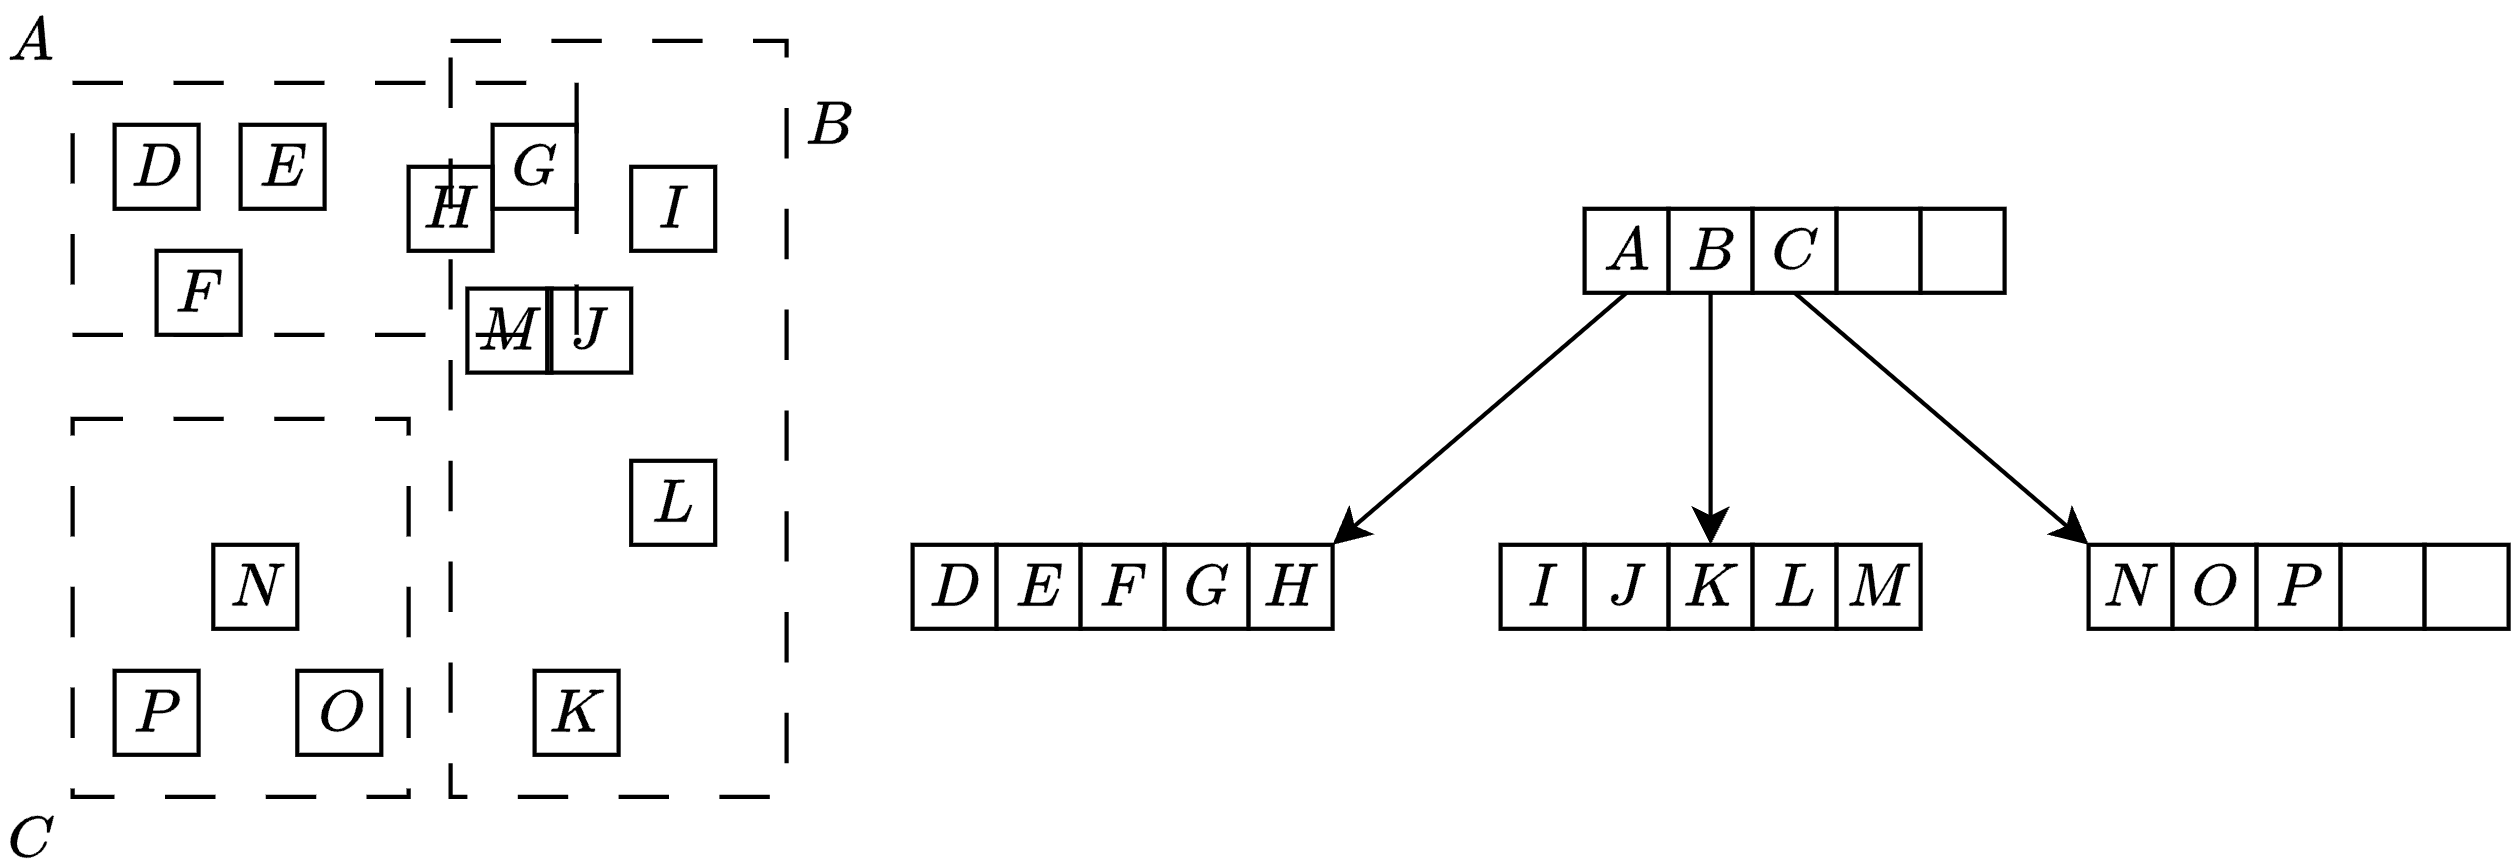
\includegraphics[width=0.5\linewidth]{images/r.png}
\end{figure}

The leaf nodes contain entries with the form $\left\langle \text{key}, \text{RID} \right\rangle$, where key stores the coordinates of the record referenced by RID. 
Actually, R-tree could also store $d$-dimensinal objects with a spatial extension, with $\text{key}=\text{MBB}(\text{object})$. 

The internal nodes contain entries of the form $\left\langle \text{MBB}, \text{PID} \right\rangle$, where MBB stores the coordinates of the MBB containing all entries reachable from the node referenced by PID. 
Overall, each node contains entries with the form $\left\langle \text{key}, \text{pointer} \right\rangle$, where key is a spatial value.

\paragraph*{Insertion}
To \texttt{insert} a new object, we start from the root and move down the tree one step at a time, trying to find a nice place where to accommodate the new object $p$. 
At each step we try to find the most suitable child node to accommodate $p$. 
In general, for each node we compute a penalty value, and choose the one with minimum penalty.
If point $p$ is inside the region of a node, then the penalty is 0. 
Otherwise, penalty can be computed as the increment of volume (area) of the MBB. 
For leaf nodes, the $R^{*}$ tree variant considers the increment of overlap with the other regions. 
Both criteria aim to obtain trees with better performance:
\begin{itemize}
    \item \textit{Large volume}: the chance of visiting the node during a query increases.
    \item \textit{Large overlap}: the number of nodes visited during a query increases.
\end{itemize}
\begin{example}
    Consider the insertion of the point $p$ in the R-tree with nodes $A$ and $B$: 
    \begin{figure}[H]
        \centering
        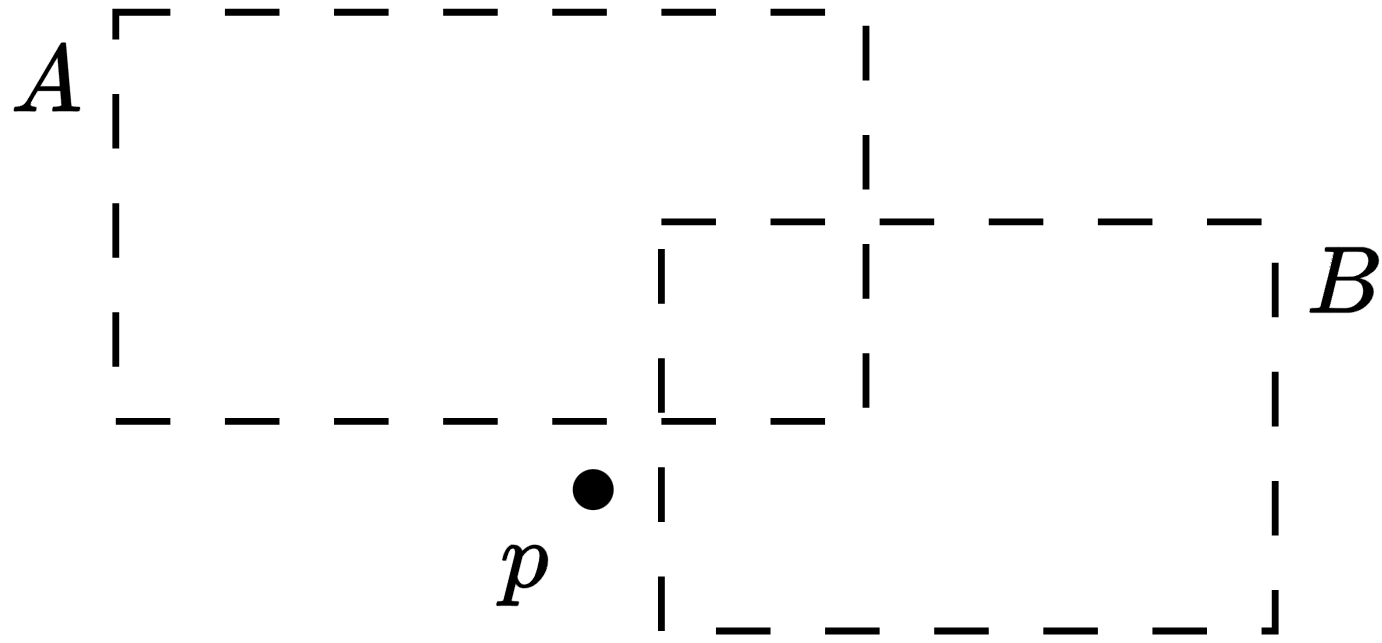
\includegraphics[width=0.4\linewidth]{images/r1.png}
    \end{figure}
    The most suitable area for the point $p$ is $B$, since the area is lower: 
    \begin{figure}[H]
        \centering
        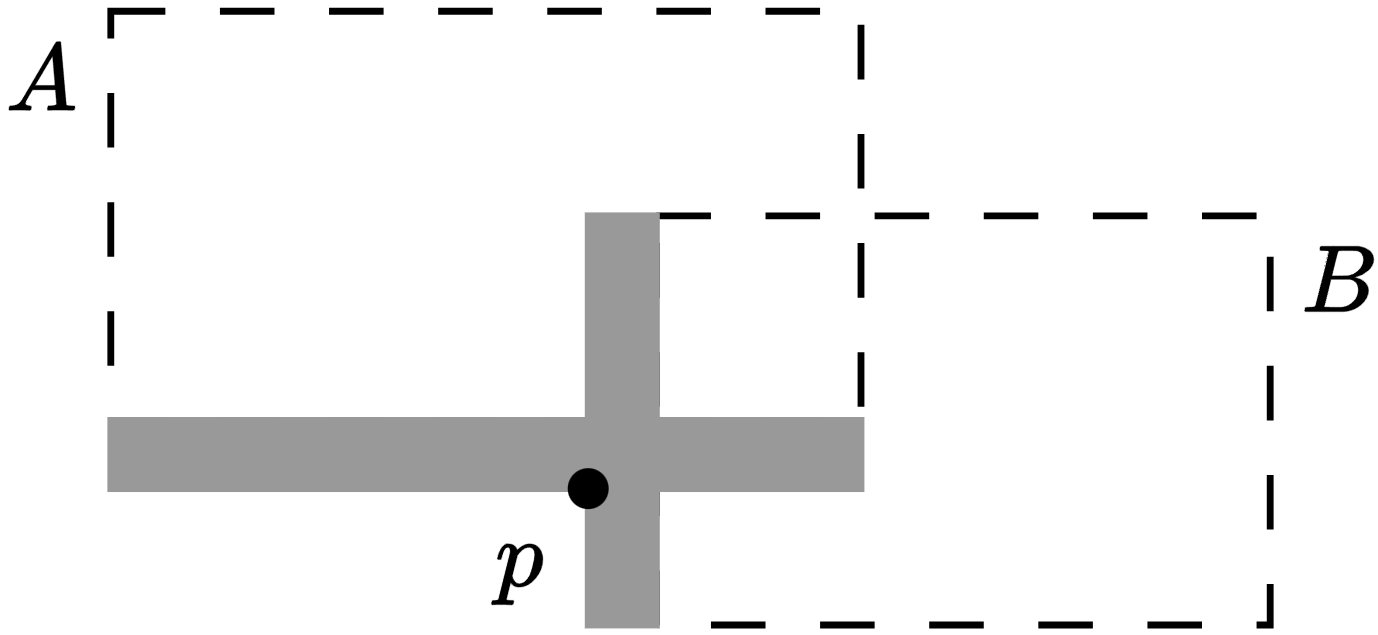
\includegraphics[width=0.4\linewidth]{images/r2.png}
    \end{figure}
\end{example}

\paragraph*{Splitting}
When $p$ has to be inserted into a leaf node $N$ that already contains $C_{\text{max}}$ entries, an overflow occurs, and $N$ has to be split. 
For leaf nodes whose entries are points the solution aims to split the set of $C_{\text{max}}+1$ points into two subsets, each with at least $C_{\text{min}}$ and at most $C_{\text{max}}$ points.
This is an $\mathcal{NP}$-hard problem, thus heuristics have to be applied. 
Among the several possibilities, one could consider the choice that leads to have a minimum overall volume. 
As in B+ trees, splits propagate upward and can recursively trigger splits at higher levels of the tree. 
The R-tree just aims to minimize the sum of resulting volumes. 
The $R^{*}$ tree implements a more sophisticated criterion, which takes into account the volume, overlap, and surface of the resulting regions.
An overlap-free split cannot be guaranteed.

\paragraph*{Search}
To search the objects we have to retrieve all points included into a product of $d$ intervals. 
Such points could only be found in nodes whose MBB overlaps with the query region. 
\begin{example}
    A visual representation of a window query in the R-tree shown in the previous example is as follows: 
    \begin{figure}[H]
        \centering
        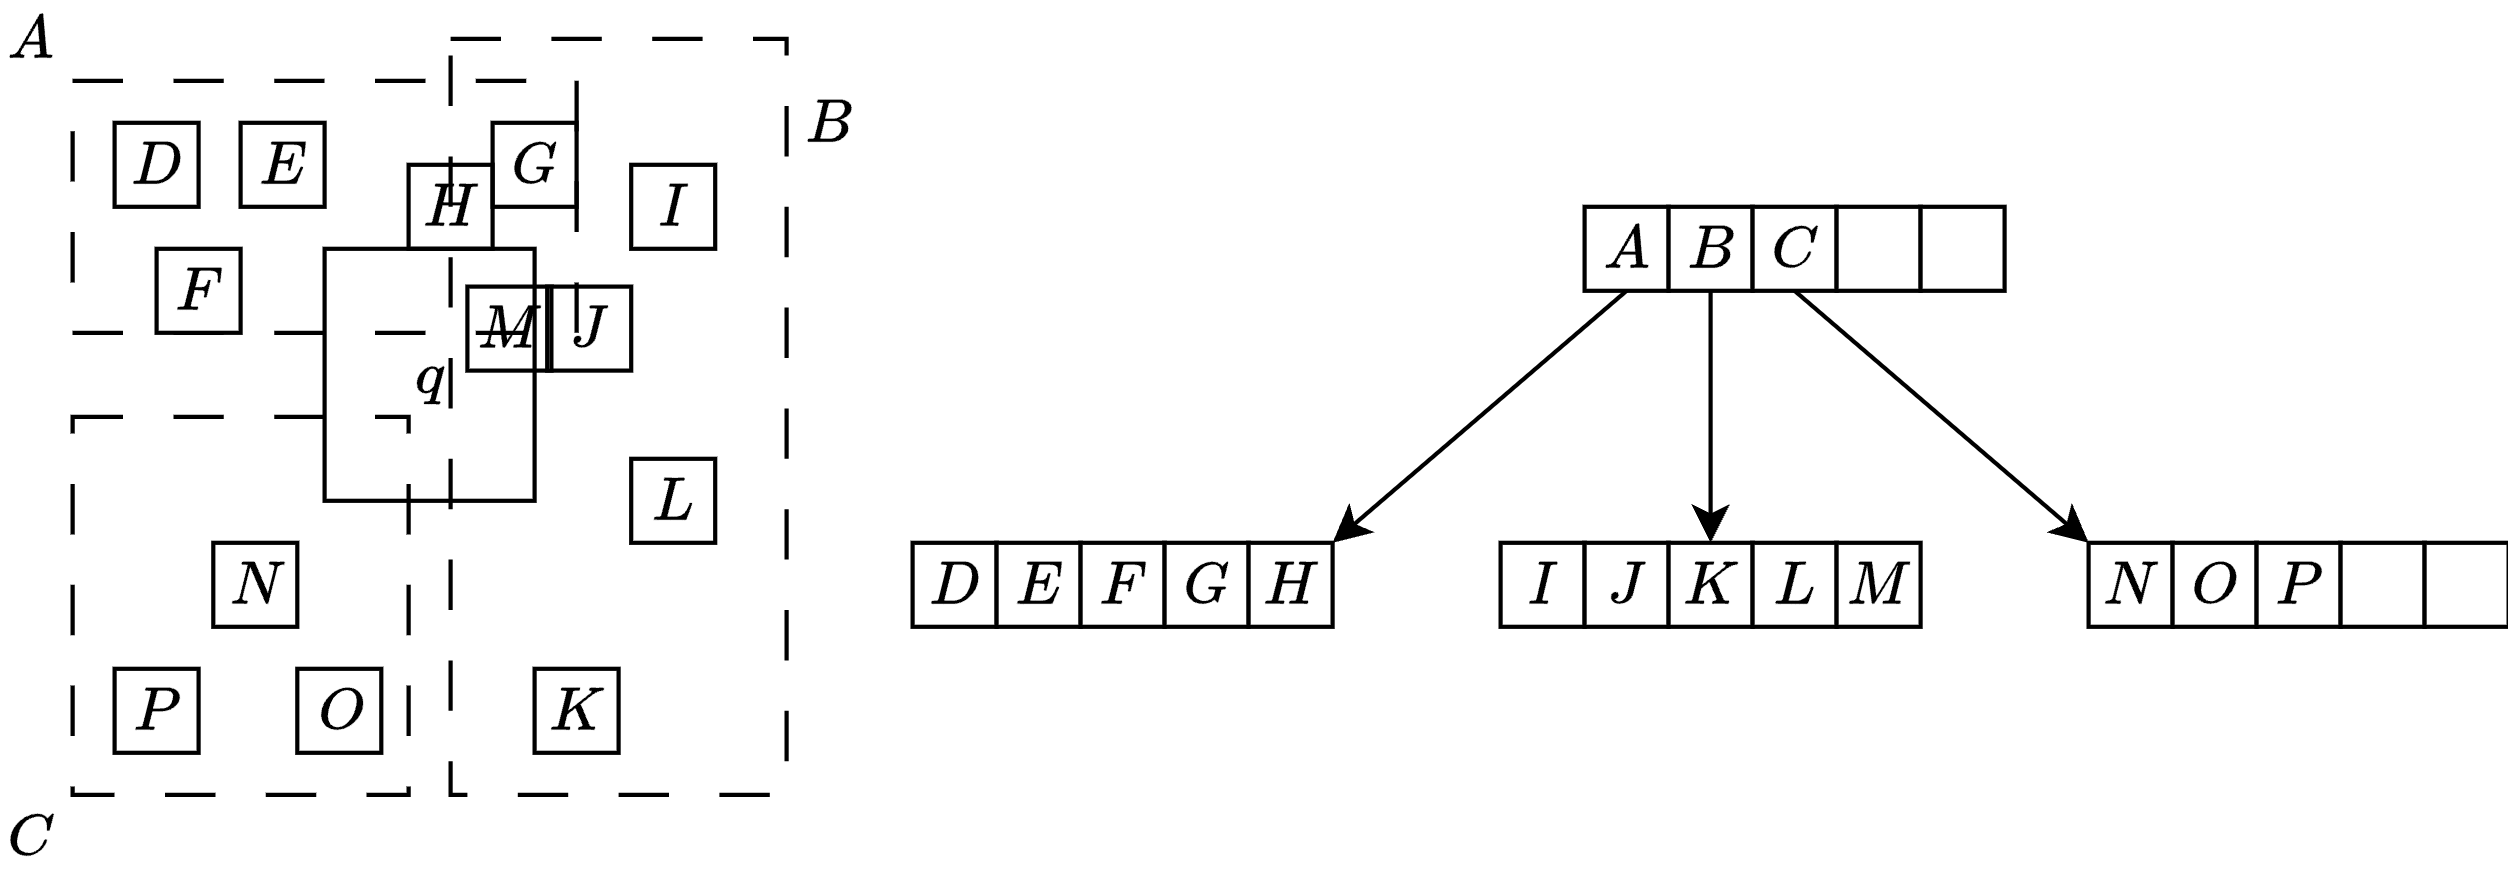
\includegraphics[width=0.5\linewidth]{images/r3.png}
    \end{figure}
\end{example}
Another possible query is the range query. 
This types of queries require: a query point $q$, a search radius $r$, and a distance function $D$.
The query region is defined as $\text{Reg}(q)=\{p|p \in \mathbb{R}^d, D(p,q) \leq r\}$. 
\begin{figure}[H]
    \centering
    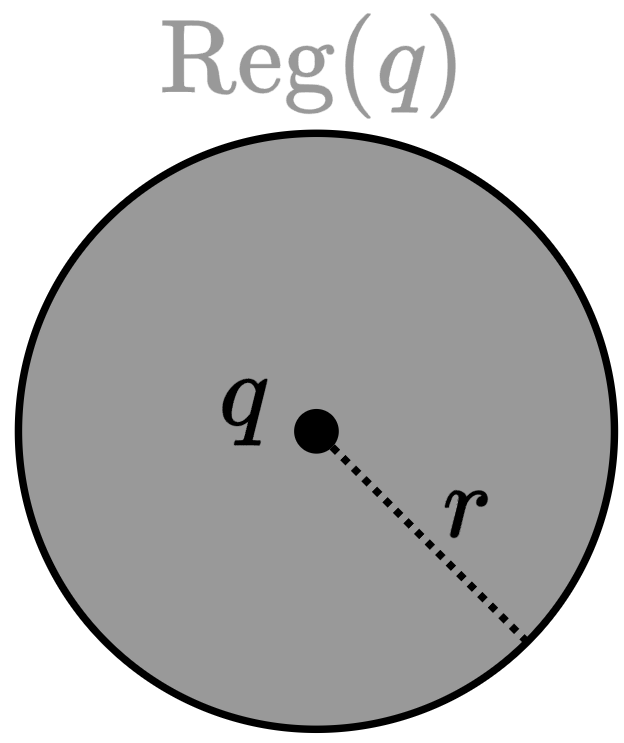
\includegraphics[width=0.15\linewidth]{images/r4.png}
\end{figure}
The algorithm for processing a range query is extremely simple:
\begin{itemize}
    \item Start from the root; for each node $N$, check if MBB($N$) intersects $\text{Reg}(q)$. 
    \item On leaf nodes, for each point $p$ check if $D(p,q) \leq r$. 
\end{itemize}

\paragraph*{Search with distance functions}
For a node $N$, we have that the minimum possible distance between $q$ and a point reachable from $N$ is: 
\[\text{D}_{\text{MIN}}(q,N)=\inf_p\{D(q,p)|p \in \text{MBB}(N)\}\]
\begin{figure}[H]
    \centering
    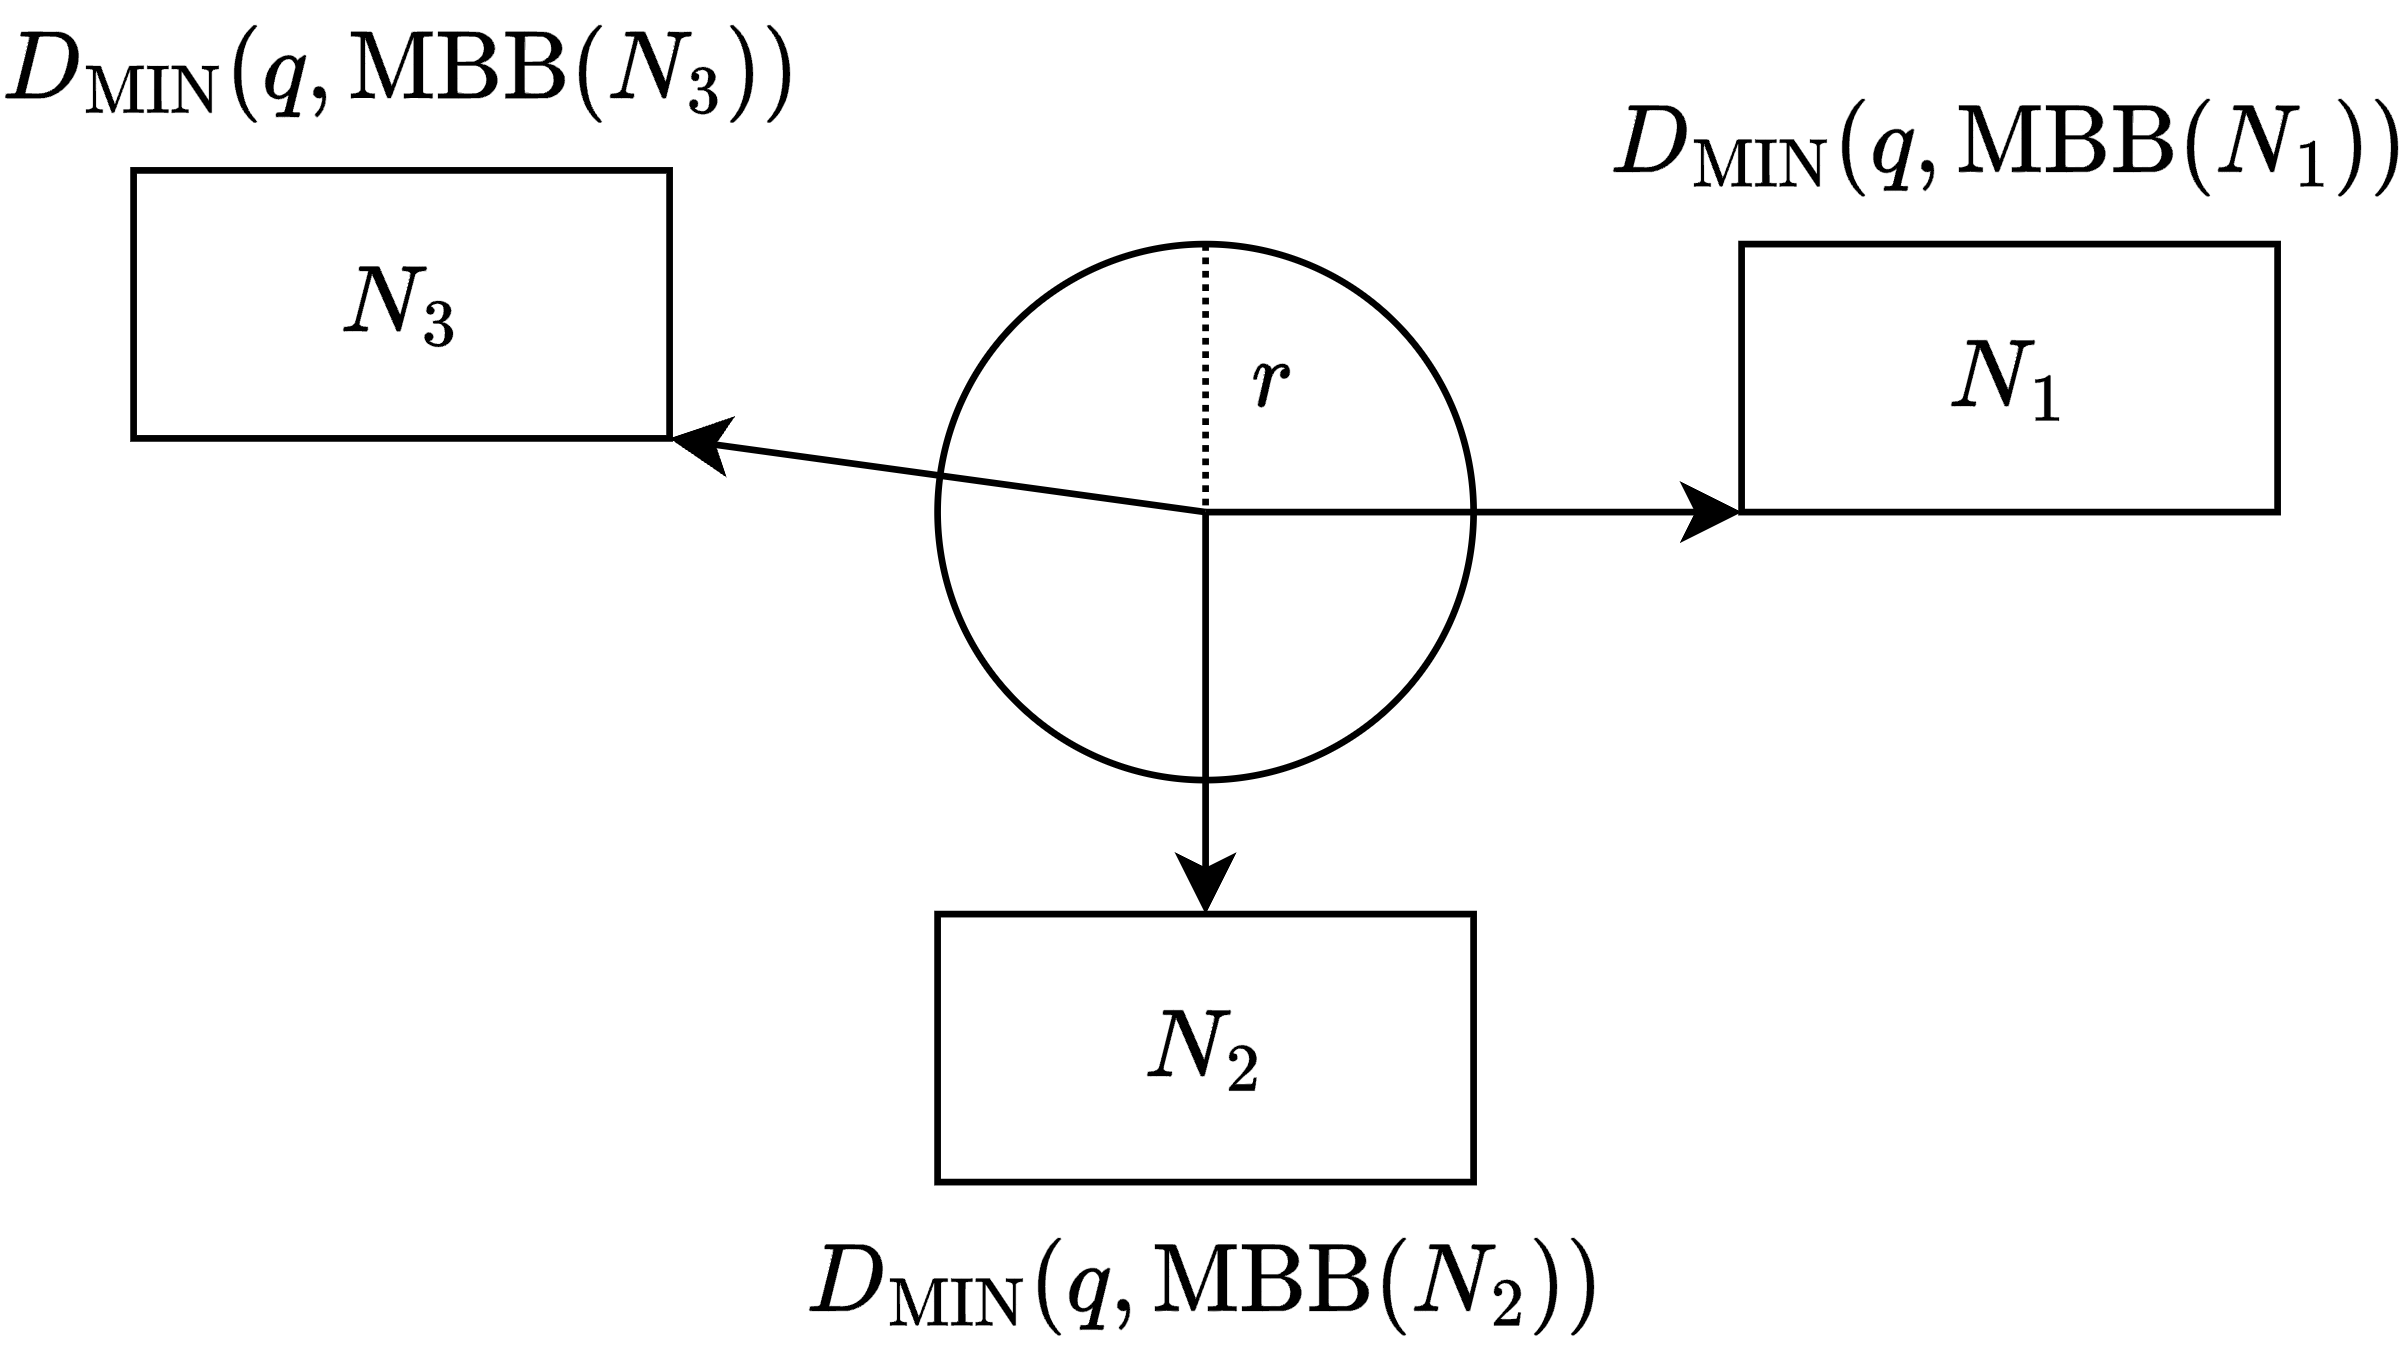
\includegraphics[width=0.5\linewidth]{images/d.png}
    \caption{Graphical representation of a general minimum distance function}
\end{figure}
The basic fact of the distance function is that: 
\[\text{Reg}(q) \cap \text{MBB}(N) \neq \varnothing \leftrightarrow \text{D}_{\text{MIN}}(q,N) \leq r\]

The most commonly used distance functions are $L_p$-norms, generally defined as: 
\[L_p(t,q)=\left( \sum_{i=1}^d \left\lvert t_i-q_i \right\rvert^p  \right)^{\frac{1}{p}}\]
Significant instances of the $L_p$-norm include:
\begin{itemize}
    \item \textit{Euclidean distance}: $L_2(t,q)=\sqrt{\sum_{i=1}^{d}{\left\lvert t_i-q_i \right\rvert^{2}}}$
    \item \textit{Manhattan distance}: $L_1(t,q)=\sum_{i=1}^{d}{\left\lvert t_i-q_i \right\rvert}$
    \item \textit{Čebyšëv distance}: $L_{\infty}(t,q)=\max_{i}\{\left\lvert t_i-q_i\right\rvert\}$
\end{itemize}
With the correspondent weighted versions: 
\begin{itemize}
    \item \textit{Euclidean distance}: $L_2(t,q)=\sqrt{\sum_{i=1}^{d}{w_i\left\lvert t_i-q_i \right\rvert^{2}}}$
    \item \textit{Manhattan distance}: $L_1(t,q)=\sum_{i=1}^{d}{w_i\left\lvert t_i-q_i \right\rvert}$
    \item \textit{Čebyšëv distance}: $L_{\infty}(t,q)=\max_{i}\{w_i\left\lvert t_i-q_i\right\rvert\}$
\end{itemize}

For the $i$-th coordinate of a given MBB let us define the offset of the query point $q=(q_1,\dots,q_d)$ with respect to $\text{MBB}(N)$ as:
\[ \delta_i=\begin{cases}
    q_i-h_i \qquad \textnormal{if } q_i \geq h_i \\
    l_i-q_i \qquad \textnormal{ if } l_i \geq q_i \\
    0 \qquad\qquad \textnormal{  otherwise}
\end{cases}\]
As a result the distance $D_{\text{MIN}}$ is computed as:
\[L_{p,\text{MIN}}(q,N;W)=\left( \sum_{i=1}^d{w_i\delta_i^p} \right)^{\frac{1}{p}}\]

\paragraph*{Search with k-NN queries}
The \texttt{kNNOptimal} algorithm can solve k-NN queries with an R-tree in an I/O-optimal way. 
The algorithm also applies to all index structures such that the region of any child node is included in the one of its parent. 

The basic case considers $k=1$. 
In such case, let $t_{NN}$ be the first nearest neighbor of $q$ $(1-NN=NN)$, and let $r_{NN}=D(q,t_{NN})$ be its distance from $q$. 
Clearly, $r_{NN}$ is only known when the algorithm terminates. 
\begin{theorem}
    Any correct algorithm for 1-NN queries must visit at least all the nodes $N$ whose $D_{\text{MIN}}$ is strictly less than $r_{NN}$, i.e., $D_{\text{MIN}}(q,N) < r_{NN}$. 
\end{theorem}
\begin{proof}
    If an algorithm A stops by reporting as $NN$ of $q$ a point $t$, and A does not read a node $N$ such that $D_{\text{MIN}}(q,N) < D(q,t)$, then $N$ might lead to a point $t^{'}$ with $D(q,t^{'}) < D(q,t)$, thus contradicting the hypothesis that $t$ is the $NN$ of $q$.
\end{proof}

kNNOptimal uses a priority queue PQ, whose elements are pairs $\left\langle \text{ptr}(N), D_{\text{MIN}}(q,N)\right\rangle $
PQ is ordered by increasing values of $D_{\text{MIN}(q,N)}$. 
This means that \texttt{dequeue} extracts from PQ the pair with minimal $D_{\text{MIN}}$ and \texttt{enqueue}($\left\langle \text{ptr}(N), D_{\text{MIN}}(q,MBB(N)) \right\rangle $) performs an ordered insertion of the pair in the queue. 
\begin{property}
    If we have found a point $t$ with $D(q,t) = r$, then all nodes $N$ with $D_{\text{MIN}}(q,N) \geq r$ can be excluded from the search. 
\end{property}
If a node can be excluded, it can be pruned. 
This operation is done with the function \texttt{update}(PQ). 
If you do not want to prune the nodes, it is possible to leave such nodes in the queue and stop when the result cannot be improved anymore. 

The input of this algorithm is a query point $q$ and an index tree with root node RN. 
The outputs are $t_{NN}$, the nearest neighbor of $q$, and $r_{NN}=D(q,t_{NN})$. 
\begin{algorithm}[H]
    \caption{kNNOptimal Algorithm}
        \begin{algorithmic}[1]
            \State Initialize PQ with $\left\langle \text{ptr}(RN),0 \right\rangle $
            \State $r_{NN}:=\infty$
            \While{$\text{PQ} \neq \varnothing$}
                \State $\left\langle \text{ptr}(N),D_{\text{MIN}}(q,N) \right\rangle := \texttt{dequeue}$
                \State read($N$)
                \If{$N$ is a leaf}
                    \For{each point $t \in N$} 
                        \If{$D(q,t) < r_{NN}$}
                            \State $t_{NN} := t$
                            \State $r_{NN} := D(q,t)$
                            \State \texttt{update}(PQ)
                        \EndIf
                    \EndFor
                \Else 
                    \For{each child node $N_c \in N$}
                        \If{$D_{\text{MIN}}(q,N_c) < r_{NN}$}
                            \State \texttt{enqueue}($\left\langle \text{ptr}(N_c),D_{\text{MIN}}(q,N_c) \right\rangle$)
                        \EndIf 
                    \EndFor
                \EndIf
            \EndWhile 
            \State \Return $t_{NN}$ and $r_{NN}$
        \end{algorithmic}
\end{algorithm}

The kNNOptimal algorithm is clearly correct
To show that it is also I/O-optimal, that is, it reads the minimum number of nodes, it is sufficient to prove the following. 
\begin{theorem}
    The kNNOptimal algorithm for 1-NN queries never reads a node $N$ whose $D_{\text{MIN}}$ is strictly larger than $r_{NN}$, i.e., $D_{\text{MIN}}(q,N) > r_{NN}$. 
\end{theorem}
\begin{proof}
    Node $N$ is read only if, at some execution step, it becomes the first element in PQ. 
    Let $N_1$ be the node containing $t_{NN}$, $N_2$ its parent node, $N_3$ the parent node of $N_2$, and so on, up to $N_h = RN$, where $h$ is the height of the tree. 
    Now observe that, by definition of $D_{\text{MIN}}$, it is:
    \[r_{NN} \geq D_{\text{MIN}}(q,N_1) \geq D_{\text{MIN}}(q,N_2) \geq \dots \geq D_{\text{MIN}}(q,N_h)\]
    At each time step before we find $t_{NN}$, one (and only one) of the nodes $N_1,N_2,\dots,N_h$ is in the priority queue. 
    It follows that $N$ can never become the first element of PQ. 
\end{proof}
The algorithm is easily extended to the case $k \geq 1$ by using: 
\begin{itemize}
    \item A data structure (Res), where we maintain the $k$ closest objects found so far, together with their distances from $q$. 
    \item A current search radius the distance, $rk-NN$, of the current $k$-th $NN$ of $q$, that is, the $k$-th element of Res.
\end{itemize}
While the rest of the algorithm remains unchanged. 

\paragraph*{Indexing regions}
Leaves can store MBB's of regions, rather than points. 
Assume you want to determine all the data regions o that are at distance less or equal to $r$ from the query region, i.e., $L2(q,o) \geq r$. 
We have to apply two phases: 
\begin{enumerate}
    \item \textit{Filter}: use the index and retrieve all the MBB's such that $L_2\left(\text{MBB}(q),\text{MBB}(o)\right) \leq r$. 
    \item \textit{Refine}: access the actual geometries of the objects and apply the test $L_2(q,o) \leq r$. 
\end{enumerate}
\begin{figure}[H]
    \centering
    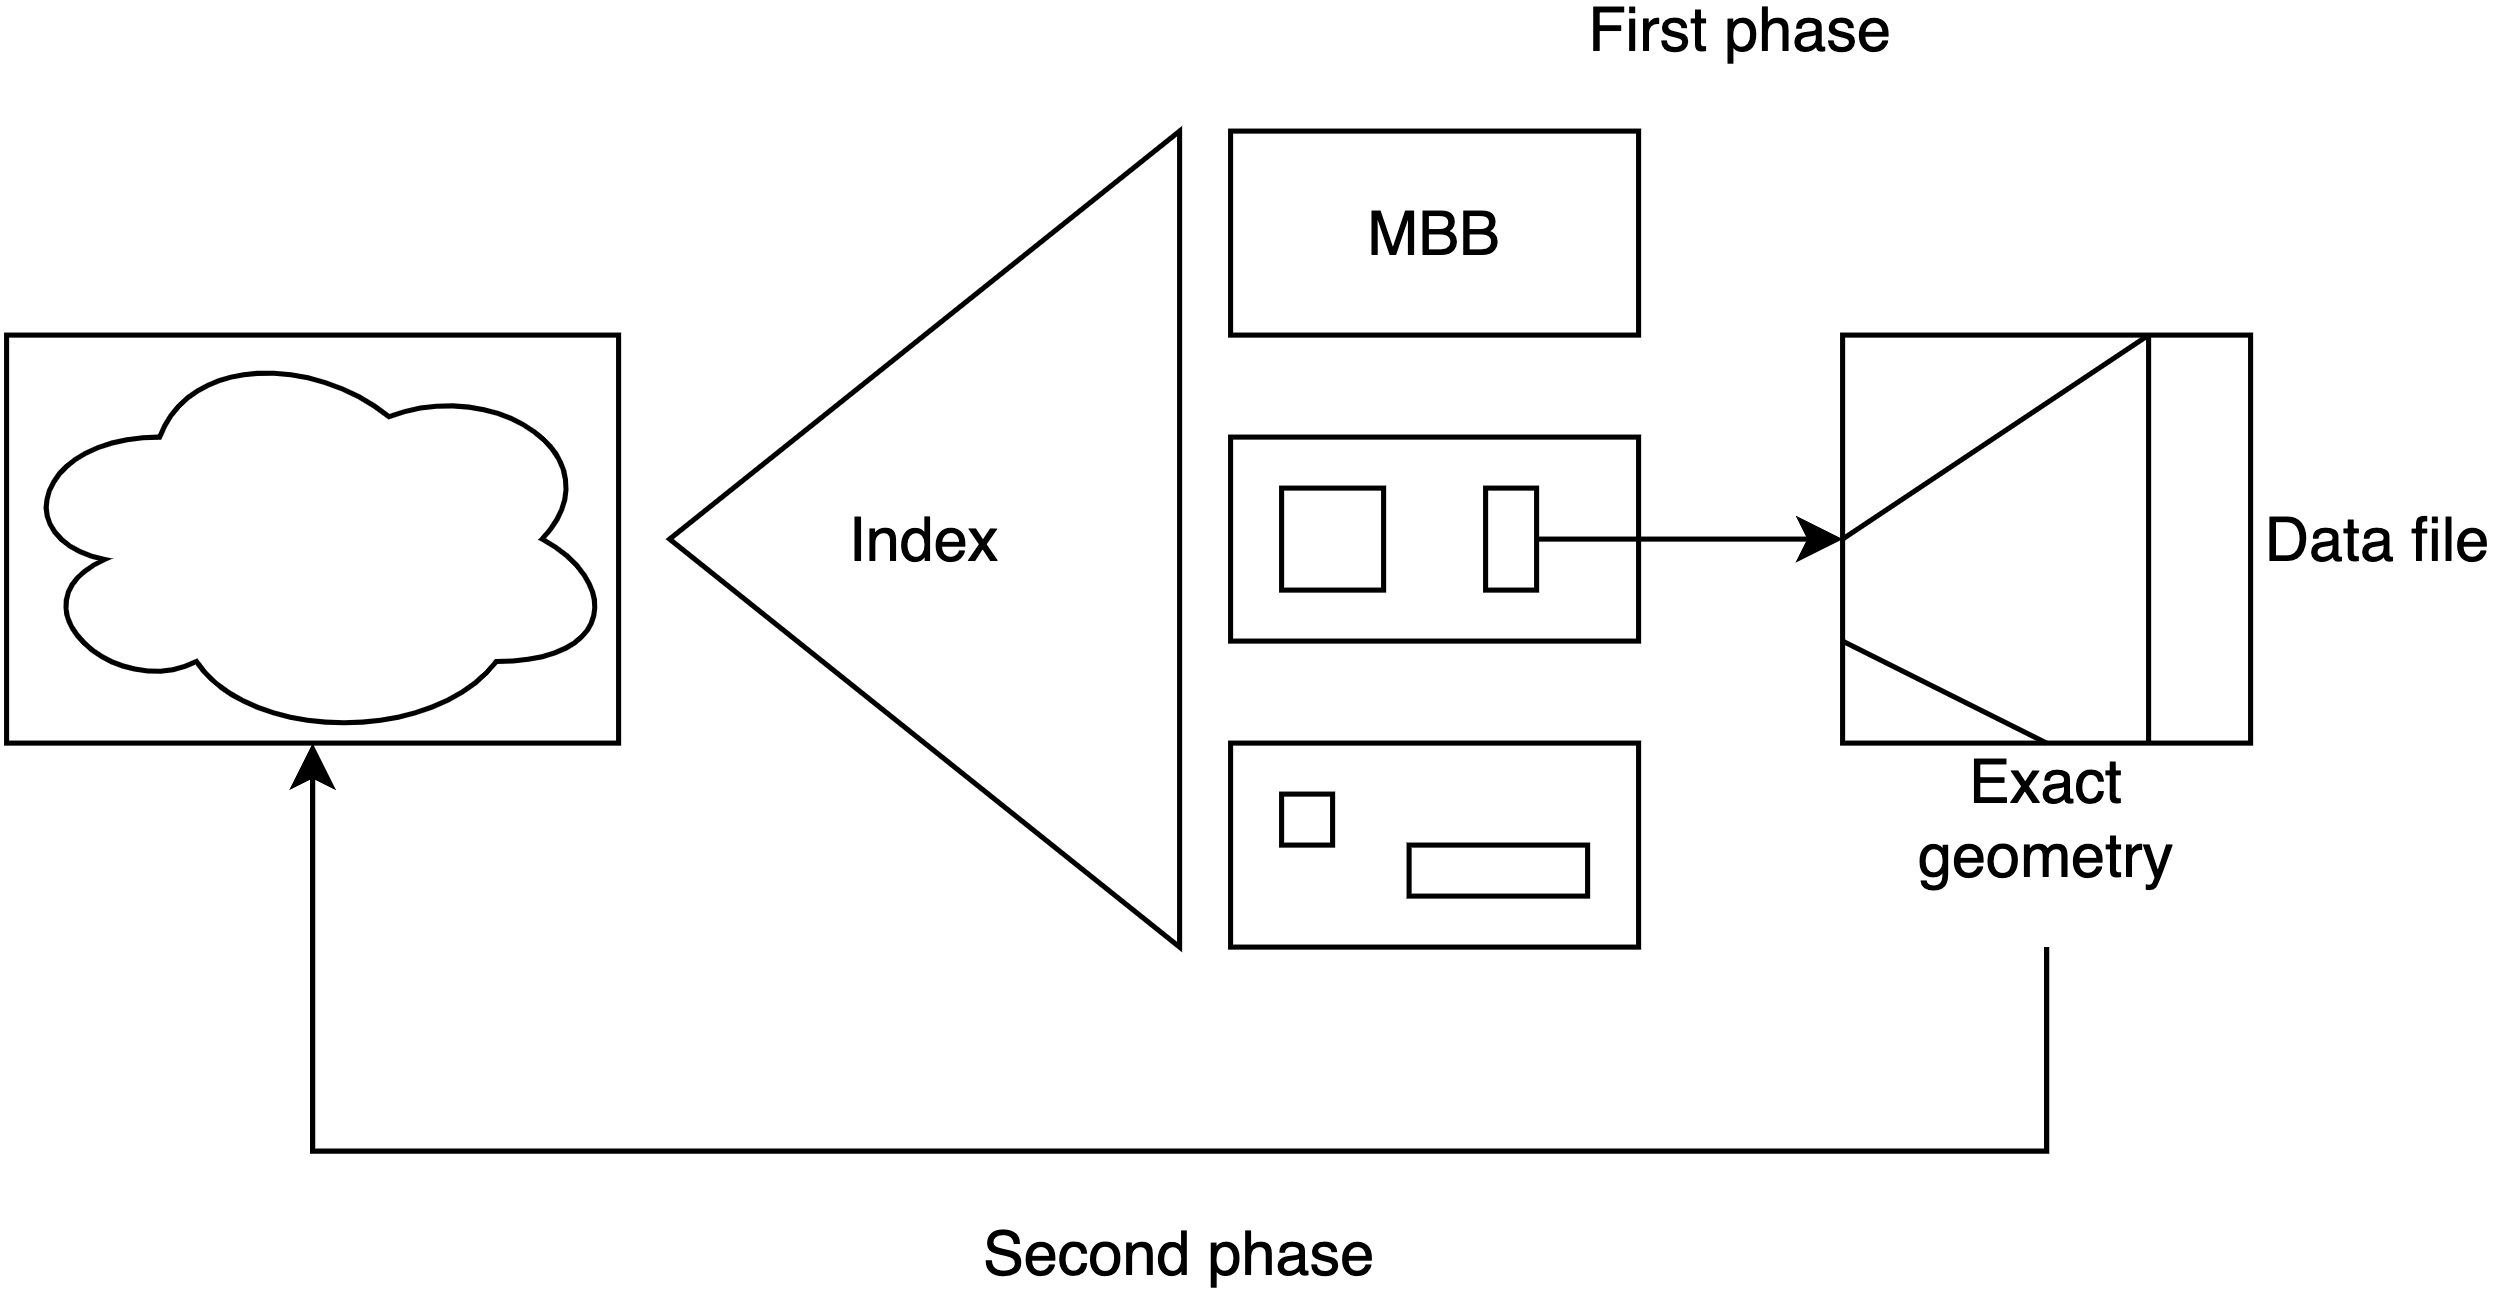
\includegraphics[width=0.5\linewidth]{images/i.png}
    \caption{Representation of indexing regions procedure}
\end{figure}